\vspace{+15pt}
\section{Auswertung}
\label{sec:Auswertung}

\vspace{+15pt}
\subsection{Vorbereitende Berechnungen}
\vspace{+5pt}

Der erste Detektorscan wird mittels Funktion 
\textit{scipy.optimize.curve\_fit} aus der Python-Bibliothek SkiPy nach der Gaußfunktion

\begin{equation}
    f(\alpha_i) = \frac{a}{\sqrt{2 \pi \sigma^2}} \text{exp}\left(- \frac{(\alpha_i - \mu)^2}{2\sigma^2}\right) + b
\end{equation}

\vspace{+10pt}
approximiert und ist in Abbildung \ref{fig:plot1} dargestellt.
Die Näherungsparameter ergeben sich zu
\vspace{-25pt}

\begin{align*}
    \mu &= (\num{-4.1 +- 0.5}) \cdot 10^{-3}\si{\degree} \; ,\\
    \sigma &= (\num{45.9 +- 0.6}) \cdot 10^{-3} \si{\degree} \; ,\\
    a &= (\num{18.55 +- 0.22}) \cdot 10^4 \; ,\\
    b &= (\num{1.6 +- 0.4}) \cdot 10^4 \; .
\end{align*}

\vspace{-7pt}
\begin{figure}[H]
    \centering
    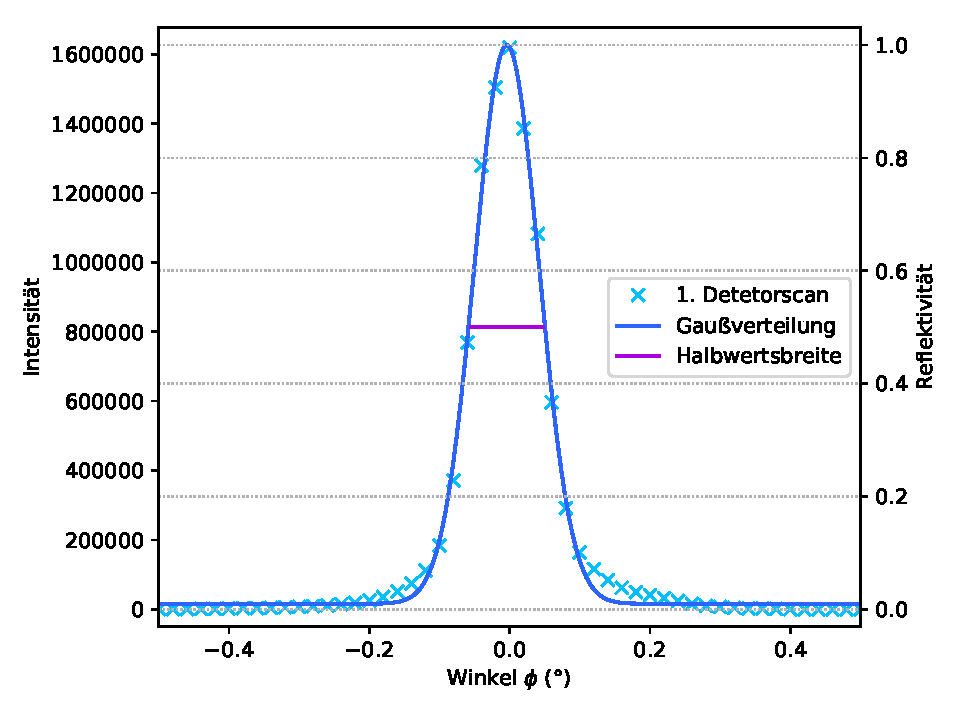
\includegraphics[scale=0.7]{content/plot1.pdf}
    \vspace{-10pt}
    \caption{Gaußgenäherte Intensität des ersten Detektorscans in Abhängigkeit des Einfallswinkels $\alpha_i$.}
    \label{fig:plot1}
\end{figure}

Aus den aufgenommenen Daten und des Maximums der Gaußnäherung ergeben sich die maximalen
Intensitäten von 
\vspace{-25pt}

\begin{align*}
    I_\text{max,detec} &= \num{1618610} \; ,\\
    I_\text{max,gauss} &= \num{1626579.26}
\end{align*}

und die Halbwertsbreite der Näherung von

\begin{equation*}
    d_{\sfrac{1}{2}} = \SI{0.12}{\degree} \; .
\end{equation*}

In Abbildung \ref{fig:plot21} ist der erste Z-Scan dargestellt.
Aus diesem lässt sich anhand der Differenz der Höhen rechts und links der negativen Flanke der Intensität
die Strahldicke als etwa

\begin{equation*}
    d_\text{S} = \SI{0.28}{\milli\meter}
\end{equation*}

bestimmen. Zudem übersteigt hier die maximale Intensität die des Detektorscans mit 

\begin{equation*}
    I_\text{max,z} = \num{1636650} \; ,
\end{equation*}

mit welcher die Reflektivitäten der folgenden Scans normiert werden sollen.

\begin{figure}[H]
    \centering
    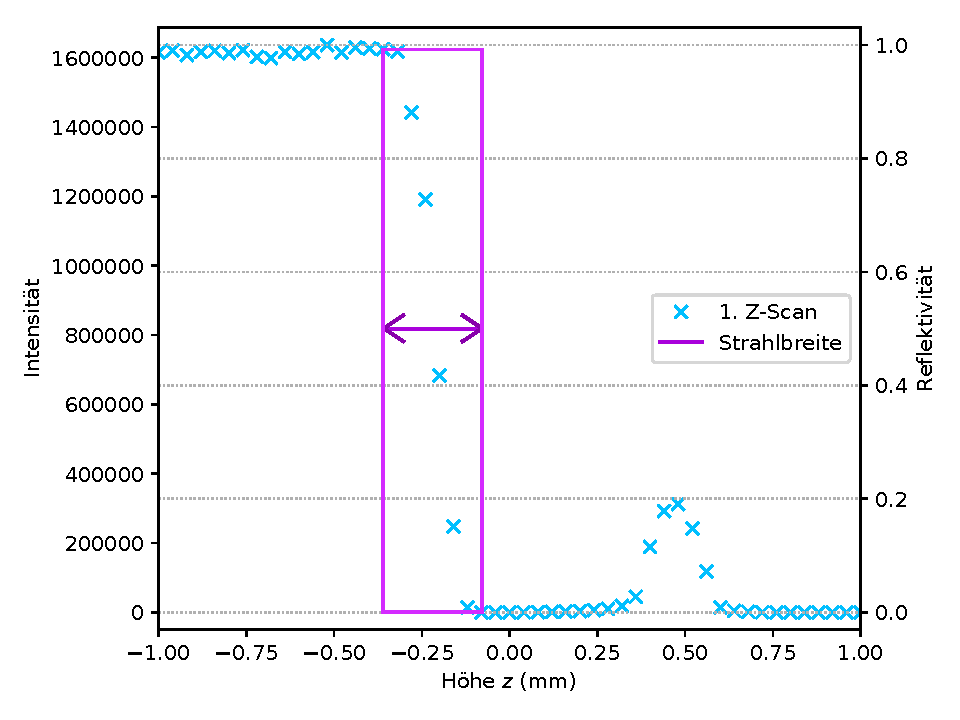
\includegraphics[scale=0.7]{content/plot21.pdf}
    \vspace{-10pt}
    \caption{Intensität des Z-Scans in Abhängigkeit der Probenhöhe $z$.}
    \label{fig:plot21}
\end{figure}

Aus dem in Abbildung \ref{fig:plot3} dargestellten ersten Rockingscans
können links und rechts des Intensitätspeaks die beiden Geometriewinkel $\alpha_{g,i}$
abgelesen werden, deren Intensitäten gerade nicht verschwindend sind. 
Zusammen mit dem gemitteltem Winkel $\alpha_g$ ergeben sich diese zu

\begin{align*}
    \alpha_{g,1} &= \SI{-0.84}{\degree} \; , \\
    \alpha_{g,2} &= \SI{0.64}{\degree} \; , \\
    \alpha_{g} = \sfrac{1}{2}|\alpha_{g,1} &- \alpha_{g,2}| = \SI{0.74}{\degree} \; .
\end{align*}

\begin{figure}[H]
    \centering
    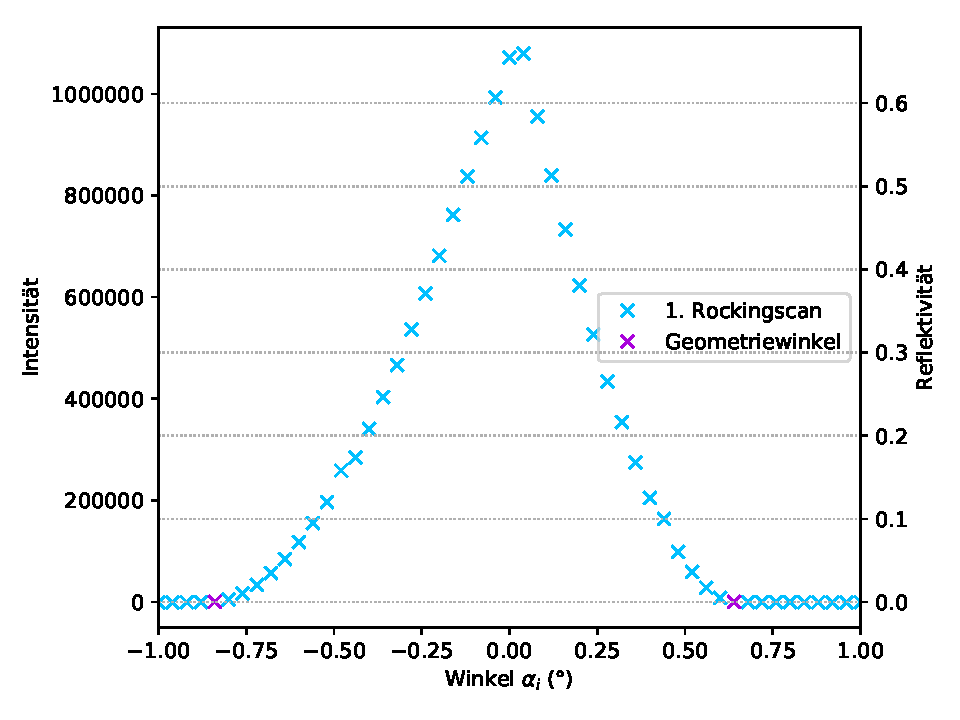
\includegraphics[scale=0.7]{content/plot3.pdf}
    \vspace{-10pt}
    \caption{Intensität des Rockingscans in Abhängigkeit des Einfallswinkels $\alpha_i$.}
    \label{fig:plot3}
\end{figure}

